\documentclass{beamer}
\usepackage[abspath]{currfile}
\usepackage{luatexja-fontspec}
\usepackage{hyperref}
\usepackage{booktabs}
\usepackage[normalem]{ulem} % either use this (simple) or

% Preamble
\usetheme{metropolis}
\setmainjfont[
  Path          = \currfileabsdir,
  UprightFont   = NotoSansCJK-Regular.ttc,
  BoldFont      = NotoSansCJK-Bold.ttc,
]{example}

\hypersetup{colorlinks,urlcolor=blue,linkcolor=black}

\newcommand{\netquote}[3]{
    \begin{block}{}
        {\textit{#1}}
        \vskip5mm
        \hspace*\fill{\small--- \href{#2}{#3}}
    \end{block}
}

\newcommand{\opinion}[1]{\item \textit{#1}\vskip5mm}
\newcommand{\opinionsby}[3]{
    \begin{block}{}
        \begin{itemize}
        #3
        \end{itemize}
        \hspace*\fill{\small--- \href{#1}{#2}}
    \end{block}
}

\newcommand{\opinionsToWord}[3]{
    \footnotesize
    \begin{itemize}
        #2
    \end{itemize}

    \onslide<#3>{
        \Large\emphasize{=> #1}
    }
}
\newcommand{\emphasize}[1]{\textcolor{red}{#1}}

\def\opCohesionA{Projects can be organized and grouped together in whatever way you find to be most logically consistent, and not just because your version control system forces you to organize things in a particular way.}
\def\opCohesionB{モノレポなら、チーム間に障壁やサイロが生じることがないので、連携性の高いマイクロサービスを設計、メンテナンスしやすくなります。}
\def\opCohesionC{[With monorepos,] If you want to report a bug and you don't know if it's caused by the server, wasm , console, or some other component, where do you submit the issue?}

\def\opMeritEfficiencyA{Tools basically just need to be able to read files.}
\def\opMeritEfficiencyB{Monorepos make local dev easy. One Git pull and run a script. All services and dependencies running from master on your machine.}
\def\opMeritEfficiencyC{リポジトリを単一化し、共通モデル、共有ライブラリ、ヘルパーコードをすべてまとめておけば、マイクロサービスが多くてもこれらを使いまわせる。}
\def\opMeritEfficiencyD{1つのPull Requestを作成するのに10分だとしても、10リポジトリを対象にすると100分かかる。}
\def\opMeritEfficiencyE{開発時に複数のリポジトリをIDEなどで開く必要がなくプロジェクト間の移動が容易。}

\def\opCouplingA{共通のコードを変更すると、数多くのアプリケーション コンポーネントに影響が及んでしまいます。ソースの競合によりマージしにくい場合もあります。}
\def\opCouplingB{チーム構造がフラットでない場合(業務委託など)の権限管理が大変。}
\def\opCouplingC{自分が関わらないコードも自分の環境下に置くこととなる。}
\def\opCouplingD{自分に関係のないコミットが打たれる。}
\def\opCouplingE{パッケージ間の依存関係が大量に発生する。}

\def\opDemeritEfficiencyA{デプロイプロセスが複雑化する可能性があり、ソース管理システムのスケーリングも必要です。}
\def\opDemeritEfficiencyB{1つの巨大なGitリポジトリを作成する事により、Gitのパフォーマンス低下が起きる可能性があります。}
\def\opDemeritEfficiencyC{関わるメンバー全員にモノレポの知識が求められる。}


% Title
\title{モノレポのすゝめ}
\author{ハララノフ ヴァレリ \and 三輪 智樹}
\institute{個人\\情報科学若手の会}
% TODO
\date{2024-09-15} % chktex 8

\begin{document}

\frame{\titlepage}

\section{はじめに}
\begin{frame}
    \frametitle{我々は・・・}
    \only<2>{・・・宇宙人だ.}\only<3>{・・・\sout{宇宙人だ.} 三輪とヴァレリだ.}
    \begin{itemize}
        \item<4-> 三輪
        \begin{itemize}
            \item<5-> 名前: みわ ともき
            \item<6-> 領域: TypeScript X Frontend
            \item<7-> 趣味: ホラー映画、音楽聴く
        \end{itemize}
        \item<8-> ヴァレリ
        \begin{itemize}
            \item<9-> foo
        \end{itemize}
    \end{itemize}
\end{frame}
\section{モノレポとは?}
\begin{frame}
\frametitle{モノレポとは? --- 定義}
    \only<2>{
        \netquote{
            A monorepo is a software-development strategy in which the code for a number of projects is stored in the same repository.
        }{http://en.wikipedia.org/w/index.php?title=Monorepo&oldid=1221537048}{Wikipedia}
    }
    \only<3>{
        \netquote{
            A monorepo is a single repository containing multiple distinct projects, with well-defined relationships.
        }{https://monorepo.tools/}{monorepo.tools}
    }
    \only<4>{
        \netquote{
            A monorepo is a single git repository that holds the source code for multiple applications and libraries, along with the tooling for them.
        }{https://nx.dev/concepts/decisions/why-monorepos}{nx.dev}
    }
\end{frame}

\begin{frame}
\frametitle{モノレポとは? --- 例えば (OSS)}
\begin{itemize}
    \item \href{https://github.com/babel/babel}{Babel}
    \item \href{https://github.com/facebook/react}{React}
    \item \href{https://github.com/yarnpkg/yarn}{Yarn}
    \item \href{https://github.com/NixOS/nixpkgs}{NixOS}
    \item \href{https://github.com/ProtonMail/WebClients}{ProtonMail}
\end{itemize}
\end{frame}

\section{To モノレポ or not to モノレポ}
\begin{frame}
    \frametitle{何が嬉しいの?}
    \only<2>{
        \opinionsby{https://danluu.com/monorepo/}{danluu.com/monorepo}{
            % 凝集度
            \opinion{\opCohesionA}
            % 大局的作業効率
            \opinion{\opMeritEfficiencyA{}}
        }
    }
    \only<3>{
        \opinionsby{https://www.reddit.com/r/ExperiencedDevs/comments/tmca5u/comment/i1xtv3b}{/r/ExperiencedDevs}{
            % 大局的作業効率
            \opinion{\opMeritEfficiencyB}
        }
    }
    \only<4>{
        \opinionsby{https://circleci.com/ja/blog/monorepo-dev-practices/}{CircleCI}{
            % 凝集度
            \opinion{\opCohesionB}
        }
    }
    \only<5>{
        \opinionsby{https://zenn.dev/mikann_mikann/scraps/6bd6b8b31bb564}{zenn.dev/mikann\_mikann}{
            % 大局的作業効率
            \opinion{\opMeritEfficiencyC}
        }
    }
    \only<6>{
        \opinionsby{https://tech.buysell-technologies.com/entry/adventcalendar2023-12-11}{tech.buysell-technologies.com}{
            % 大局的作業効率
            \opinion{\opMeritEfficiencyD}
        }
    }
    \only<7>{
        \opinionsby{https://hireroo.io/journal/tech/mono-repo-for-microservices}{hireroo.io}{
            % 大局的作業効率
            \opinion{\opMeritEfficiencyE}
        }
    }
    \only<8>{
        \opinionsby{https://medium.com/streamdal/mostly-terrible-the-monorepo-5db704f76bdb}{medium.com/streamdal}{
            % 凝集度
            \opinion{\opCohesionC}
        }
    }
\end{frame}

\begin{frame}
    \frametitle{何がめんどいの?}
    \only<2>{
        \opinionsby{https://circleci.com/ja/blog/monorepo-dev-practices/}{CircleCI}{
            % 結合度
            \opinion{\opCouplingA}
            % パフォ効率
            \opinion{\opDemeritEfficiencyA}
        }
    }
    \only<3>{
        \opinionsby{https://tech.buysell-technologies.com/entry/adventcalendar2023-12-11}{tech.buysell-technologies.com}{
            % パフォ効率
            \opinion{\opDemeritEfficiencyB}
        }
    }
    \only<4>{
        \opinionsby{https://buildersbox.corp-sansan.com/entry/2024/05/27/110000}{buildersbox.corp-sansan.com}{
            % 結合度
            \opinion{\opCouplingB}
        }
    }
    \only<5>{
        \opinionsby{https://kk-web.link/blog/20210507}{kk-web.link}{
            % 結合度
            \opinion{\opCouplingC}
            % 結合度
            \opinion{\opCouplingD}
            % 結合度
            \opinion{\opCouplingE}
            % パフォ効率
            \opinion{\opDemeritEfficiencyC}
        }
    }
\end{frame}

\section{TODO: 分析タイトル}

\begin{frame}
    \frametitle{分析}
    \opinionsToWord{凝集度}{
        \item<2-> \opCohesionA
        \item<3-> \opCohesionB
        \item<4-> \opCohesionC
    }{5}
\end{frame}

\begin{frame}
    \frametitle{分析}
    \opinionsToWord{作業効率}{
        \item<2-> \opMeritEfficiencyA
        \item<3-> \opMeritEfficiencyB
        \item<4-> \opMeritEfficiencyC
        \item<5-> \opMeritEfficiencyD
        \item<6-> \opMeritEfficiencyE
    }{7}
\end{frame}

\begin{frame}
    \frametitle{分析}
    \opinionsToWord{結合度}{
        \item<2-> \opCouplingA
        \item<3-> \opCouplingB
        \item<4-> \opCouplingC
        \item<5-> \opCouplingD
        \item<6-> \opCouplingE
    }{7}
\end{frame}

\begin{frame}
    \frametitle{分析}
    \opinionsToWord{作業効率}{
        \item<2-> \opDemeritEfficiencyA
        \item<3-> \opDemeritEfficiencyB
        \item<4-> \opDemeritEfficiencyC
    }{5}
\end{frame}

\begin{frame}
    \frametitle{異議あり!論点を掘り下げてみよう!}
    \begin{block}{}
        \centering
        \begin{tabular}{cc}
            \toprule
            メリット & デメリット \\
            \midrule
            \only<1>{凝集度}\only<2>{\textcolor{red}{凝集度}} & \only<1>{結合度}\only<2>{\textcolor{red}{結合度}} \\
            作業効率 & 作業効率 \\
            \bottomrule
        \end{tabular}
    \end{block}
\end{frame}

\begin{frame}
    \frametitle{モノレポとポリレポ --- 凝集度と結合度}
    \only<2-3>{
        \onslide<2-3>{
            \begin{block}{凝集度}
                {\textit{単一\textcolor{red}{モジュール内}の要素間の関連性についての尺度。}}
            \end{block}
        }
        \onslide<3>{
            \begin{block}{結合度}
                {\textit{\textcolor{red}{モジュール間}の関連性についての尺度。}}
            \end{block}
        }
    }
    \only<4->{
        \begin{block}{凝集度}
            {\textit{単一\textcolor{red}{レポジトリ内}の要素間の関連性についての尺度。}}
        \end{block}
        \begin{block}{結合度}
            {\textit{\textcolor{red}{レポジトリ間}の関連性についての尺度。}}
        \end{block}
    }
    \onslide<3>{
        \vskip5mm
        \hspace*\fill{\small--- \href{https://www.ogis-ri.co.jp/otc/hiroba/technical/Cohesion_Coupling/Cohesion_Coupling.html}{オージス研}}
    }
\end{frame}

\begin{frame}
    \frametitle{モノレポとポリレポ --- 作業効率}
    \centering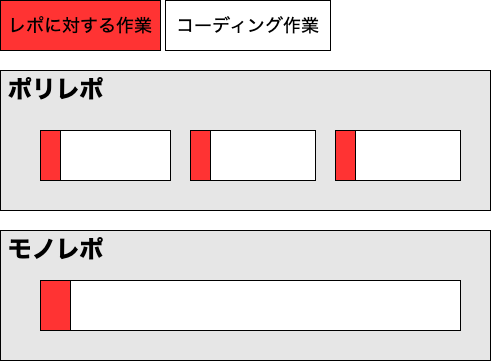
\includegraphics[height=150pt]{efficiency.png}
\end{frame}

% \begin{frame}
%     \frametitle{異議あり!論点を掘り下げてみよう!}
%     \begin{itemize}
%         \item No overhead to create new projects --- 「PJ」 と 「レポ」を混同してない?
%         \item Shared code and visibility --- どうやってシェアするの?ライブラリ?直接参照?それ,モノレポじゃなくてもできるくない?
%         \item Atomic commits across projects --- 実は異議なし.それは本当にそう.だけど,誤解しちゃだめ (lockstep リリース)
%         \item One version of everything --- それ本当に良いことなのか?
%     \end{itemize}
% \end{frame}
\section{To モノレポ or not to モノレポ?}

\begin{frame}
    \frametitle{どういうときにモノレポが良いのか?}
    \small
    \begin{block}{大前提}
        \begin{enumerate}
            \item<2-> 関係あるもの同士を同じ個体にまとめるのは管理コストを下げる.
            \item<3-> 個体を分割することは管理コストを上げる.
            \item<4-> 現実的に管理可能な個体の規模には限度がある.
        \end{enumerate}
    \end{block}
    \onslide<5>{
        \Large\emphasize{=> 上限を超えない限りモノレポが良い.}
    }
\end{frame}

\begin{frame}
    \frametitle{じゃ,どういうときにモノレポを分けるべきか?}
    会社のコードをすべて同じレポに入れたらどうなる?
    \begin{itemize}
        \item<2-> 人間による制約
        \begin{itemize}
            \item<3-> PR の処理が速すぎて追いつかない
            \item<4-> 情報が多すぎて整理できない (認知負荷が高い)
        \end{itemize}
        \item<5-> 人間以外による制約
        \begin{itemize}
            \item<6-> レポが重すぎて開けない
            \item<7-> 局所的に作業するツールがない
            \item<8-> Git そのものが落ちる
        \end{itemize}
        \item<9-> 人工的な制約
        \begin{itemize}
            \item<10-> 法律,監査要件等
        \end{itemize}
    \end{itemize}
    \onslide<11>{
        \emphasize{現実の上限にぶち当たるから分けるべき.}
    }
\end{frame}

\begin{frame}
    \frametitle{どうやって分けるか?}
    例えばこういう状況を想像してみよう
    \begin{itemize}
        \item<2-> MV 株式会社が2個のサービスを提供する
        \item<3-> サービス \textcolor{red}{A} はチーム \textcolor{red}{A},サービス \textcolor{green}{B} はチーム \textcolor{green}{B} が開発している.
        \item<5-> チーム \textcolor{red}{A} と \textcolor{green}{B} はお互いに独立 (名前も顔も知らない).
        \item<6-> サービス \textcolor{red}{A} のコードとサービス \textcolor{green}{B} のコードは同じモノレポ \textcolor{blue}{C} 内にある.
        \item<7-> サービス \textcolor{red}{A} もサービス \textcolor{green}{B} もそれぞれ front-end と back-end から成る.
    \end{itemize}
    \onslide<8>{
        \normalfont
        \begin{block}{練習問題}
            レポ \textcolor{blue}{C} が大きくなりすぎてもうモノレポのままじゃ無理そうで分割しなければならない.どのように分割するか?
        \end{block}
    }
\end{frame}

\section{モノレポから学ぶポリレポの組み方}

\begin{frame}
    \frametitle{どうやって分けるのか?}
    \begin{enumerate}
        \item<2-> サービス \textcolor{red}{A} をレポ \textcolor{red}{A} に,サービス \textcolor{green}{B} をレポ \textcolor{green}{B} に移行する.
        \item<3-> それぞれのサービスの front-end をレポ \textcolor{blue}{C\textsubscript{1}} に, back-end をレポ \textcolor{blue}{C\textsubscript{2}} に移行する.
        \item<4-> (その他)
    \end{enumerate}
    \onslide<5>{
        \Large\emphasize{=> そりゃ 1. だろ.}
    }
\end{frame}

\begin{frame}
    \frametitle{なぜそう分けるのか?}
    \begin{itemize}
        \item<2-> サービスで分けた方が,関係するもの同士だけで固まる
        \begin{itemize}
            \item<3-> \emphasize{凝集度が上がる}
        \end{itemize}
        \item<4-> 同じく,関係ないものが分かれる
        \begin{itemize}
            \item<5-> \emphasize{結合度が下がる}
        \end{itemize}
        \item<6-> 何より,開発者にとっては楽.
    \end{itemize}
\end{frame}

\begin{frame}
    \frametitle{コンポーネントごとに分けるのはだめなのか?}

    \begin{itemize}
        \item<2-> front-end 同士のレポと back-end 同士のレポ
        \begin{itemize}
            \item<3-> そういえば・・・
            \item<4-> \href{https://github.com/ProtonMail/WebClients}{ProtonMail}
            \item<5-> モノレポをモノレポに分けるッテコト?
        \end{itemize}
        \item<6-> 何が悪いのか?
        \item<7-> 依存関係を正しく組めば実現可能
    \end{itemize}
\end{frame}

\section{大結論}

\begin{frame}
    \frametitle{結局「レポ」って何?}
    \begin{itemize}
        \item<2-> レポはあくまでも箱.
        \item<3-> おもちゃごとに箱を用意するのは無駄な手間.
        \item<4-> 一緒に遊ぶおもちゃは同じ箱に入れた方が良い.
        \item<5-> おもちゃは絡まないように管理しよう.
        \item<6-> \emphasize{大事なのは「箱」ではなく「おもちゃ」である.}
    \end{itemize}
\end{frame}


\end{document}